\newpage
\part{Makromolekyler}
    \section{Redegør for opbygning af de makromolekyler der findes i fødevarer.}
        Der er 4 forskellige makromolekyler i fødevarer, nemlig kulhydrater, proteiner, fedtstoffer, og nukleinsyrer. Jeg vil mest komme ind på de 3 første. 
        \subsection{Lipider (fedtstoffer)}
           Den normale måde at indtage fedt på er ved triglycerid. Fedt er vigigt for kroppen da det er en energi kilde. Fedt er også vigtigt for kroppen da det er med til at danne cellemembranen. Fedt er også med til at danne hormoner. 
        \subsection{Kulhydrater}

        \subsection{Protein}
            Når man taler om at skulle have store guns så skal man have gains. Når man taler om gains taler man om både proteiner og kulhydrater. Men hvad er proteiner? Proteiner er et stort molekyle ligesom glucose. Proteiner er opbygget af aminosyre der findes 20 forskellige aminosyre som kan kombineres på utailige måder. Denne kæde af aminosyre kaldes også for et peptid. bindningerne mellem aminosyrerne kaldes for peptidbindinger. Læs mere om  peptidbindinger i afsnit \ref{fig:peptidbindinger}. Der findes 4 proteinstrukture
            \begin{itemize}
                \item Primærstruktur (1 - struktur)
                \item Sekundærstruktur (2 - struktur)
                \item Tertiærstruktur (3 - struktur)
                \item Kvartærstruktur (4 - struktur)
            \end{itemize}
            \textbf{Primærstruktur} er den struktur som er den simpleste.
            En normal kæde af aminosyre er primær, det der intificere at det er primærstruktur er at Den starter med \begin{math}NH_2\end{math} og slutter med en syregruppe \begin{math}COOH\end{math}.
            \textbf{Sekundærstruktur} er den stuktur som man kalder for Alpha helix og er den struktur som er foldet om sig selv som en spiral. Den Sekundærstruktur findes også som beta foldeblad. Beta foldebald er en slags siksak struktur. Der er også en beta vendning. Denne struktur binder de andre strukturer sammen.
            \textbf{Tertiærstruktur} er den rummelige opbygning af Beta foldebald, Beta vendning og Alpha helix. For at holde den rummelige opbygning sammen er der nogle svolvbroer. (cystein \begin{math}HS\end{math})
           \textbf{Kvartærstruktur} det er en samling af små proteiner det kunne være: Hemoplin, den består af 4 små proteiner. Altså protein kompleks som af flere mindre proteiner


\section{Hvilke funktioner har de forskellige makromolekyler i en organisme?}
\section{Diskuter kostens betydning i forhold til sundhed. Inddrag øvelsen om kulhydrater i fødevarer}
\section{Mere info}
\begin{figure}
    \centering
    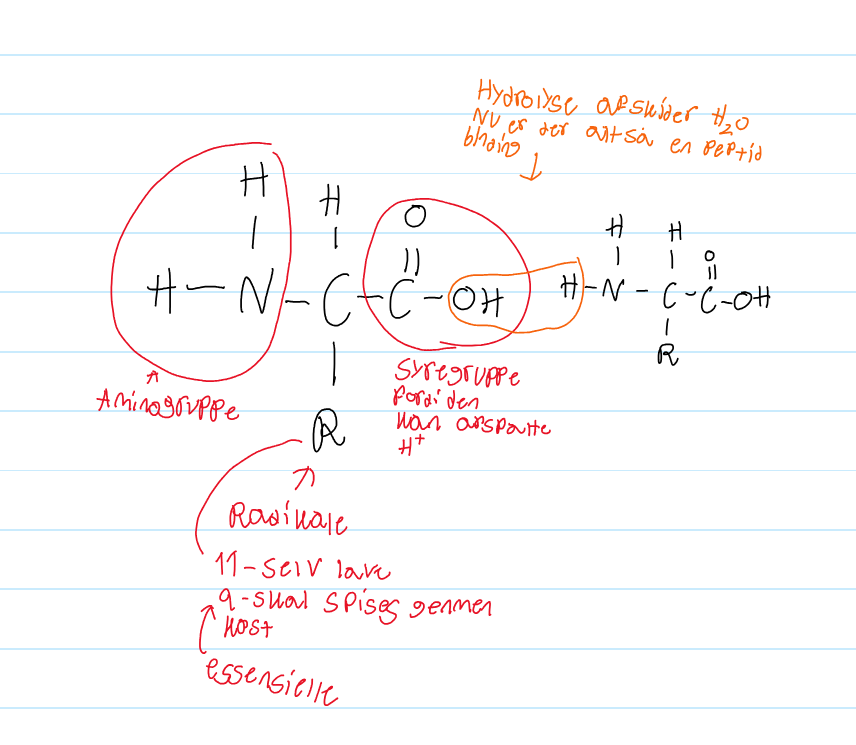
\includegraphics[width=0.8\textwidth]{figurs/peptidbindinger.png}
    \caption{Peptidbindinger}
    \label{fig:peptidbindinger}
\end{figure}